\documentclass[12pt]{article}
\usepackage{amssymb, amsmath,amsfonts}
\usepackage{tikz}
\usepackage{pgfplots}
\usepackage[pdftex, bookmarks=true,colorlinks,linkcolor=red,urlcolor=blue,citecolor=blue]{hyperref}
\usepackage{tikz}

\begin{document}

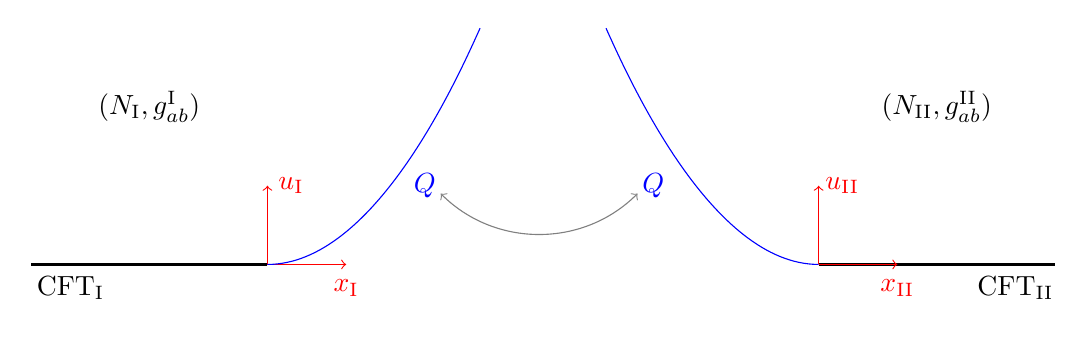
\begin{tikzpicture}
\draw[very thick] plot coordinates {(-3,0)(0,0)};
\node at (-2.5,-0.3) {CFT$_\text{I}$};

\draw[color=red] [->] (0,0) -- (1,0);
\draw[color=red]  [->] (0,0) -- (0,1);

\node[color=red] at (1,-0.3) {$x_\text{I}$};
\node[color=red] at (0.3,1) {$u_\text{I}$};
\draw[color=blue] (0,0) parabola (2.7,3);  
\draw[color=blue] (7,0) parabola (4.3,3);  
\draw[very thick] plot coordinates {(7,0)(10,0)};
\node at (9.5,-0.3) {CFT$_\text{II}$};
\draw[color=red] [->] (7,0) -- (8,0);
\draw[color=red] [->] (7,0) -- (7,1);
\node[color=red] at (8,-0.3) {$x_\text{II}$};
\node[color=red] at (7.3,1) {$u_\text{II}$};
\node at (-1.5,2) {$(N_\text{I},g^\text{I}_{ab})$};
\node at (8.5,2) {$(N_\text{II},g^\text{II}_{ab})$};
\node[color=blue] at (2,1.0) {$Q$};
\node[color=blue] at (4.9,1.0) {$Q$};
\draw[color=gray] [<->] (2.2,0.9)  to [out=-45, in=-135] (4.7,0.9);
\end{tikzpicture}

\end{document}